\chapter{Dispense 101}

% How to use Dispense.

At the same time as you set up your account, you will also have your dispense account set up. Dispense is the program that allows users to store credit and purchase items from the coke/snack machines (which are almost always cheaper than what you would find elsewhere on campus). Coke members can help you add credit to your dispense account. Call out for one in the clubroom if need be, there's always one around.


The easiest way to dispense a drink is probably the web interface (Figure \ref{webdispense.png}). Simply enter your username and password and then select a drink. 

Due to technical reasons, snacks cannot be dispensed using this interface. Getting a snack will involve typing a 5 digit User ID and a 4 digit PIN into the keypad. This allows you to dispense both drinks and snacks.

You can also use your Student Card or SmartRider as a log in device on the snack machine. To do so, log in to the Snack Machine and hold whichever card you want to use up to the card scanner (it's the thing with the blinking green light) and the card should auto- enroll. To log in using the card, simply hold the enrolled card up to the card scanner.


You can also access Dispense via shell login and using the \shell{dispense} command. Dispense isn't installed on clubroom machines so you will have to use \shell{ssh} to access one of UCC's servers.

\begin{figure}[H]
	\centering
	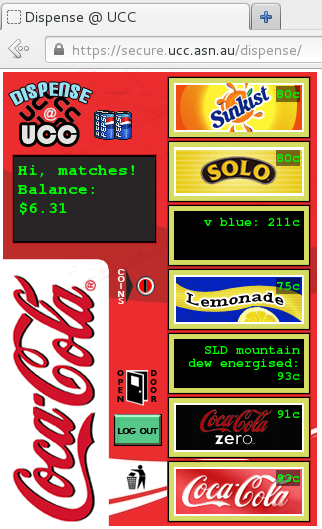
\includegraphics[width=0.5\textwidth]{figures/webdispense.png}
	\caption{The web dispense interface at \url{https://secure.ucc.asn.au/dispense}} 
	\label{webdispense.png}
\end{figure}
